\section{The Four-Role Architecture}
\label{sec:architecture}

Argus runs four persistent roles. Three of them --- Planner, Engineer, and
Reviewer --- form a numbered execution spine (L4, L1, L2). The fourth, the
Manager, deliberately sits outside that numbering because it spans the whole
pipeline rather than occupying a station on it. A fifth role, the Curator, is
optional and runs only in team/subagent modes. The schematic in Figure~1
shows how the roles sit over the domain-agnostic harness.

\begin{figure}[t]
\centering
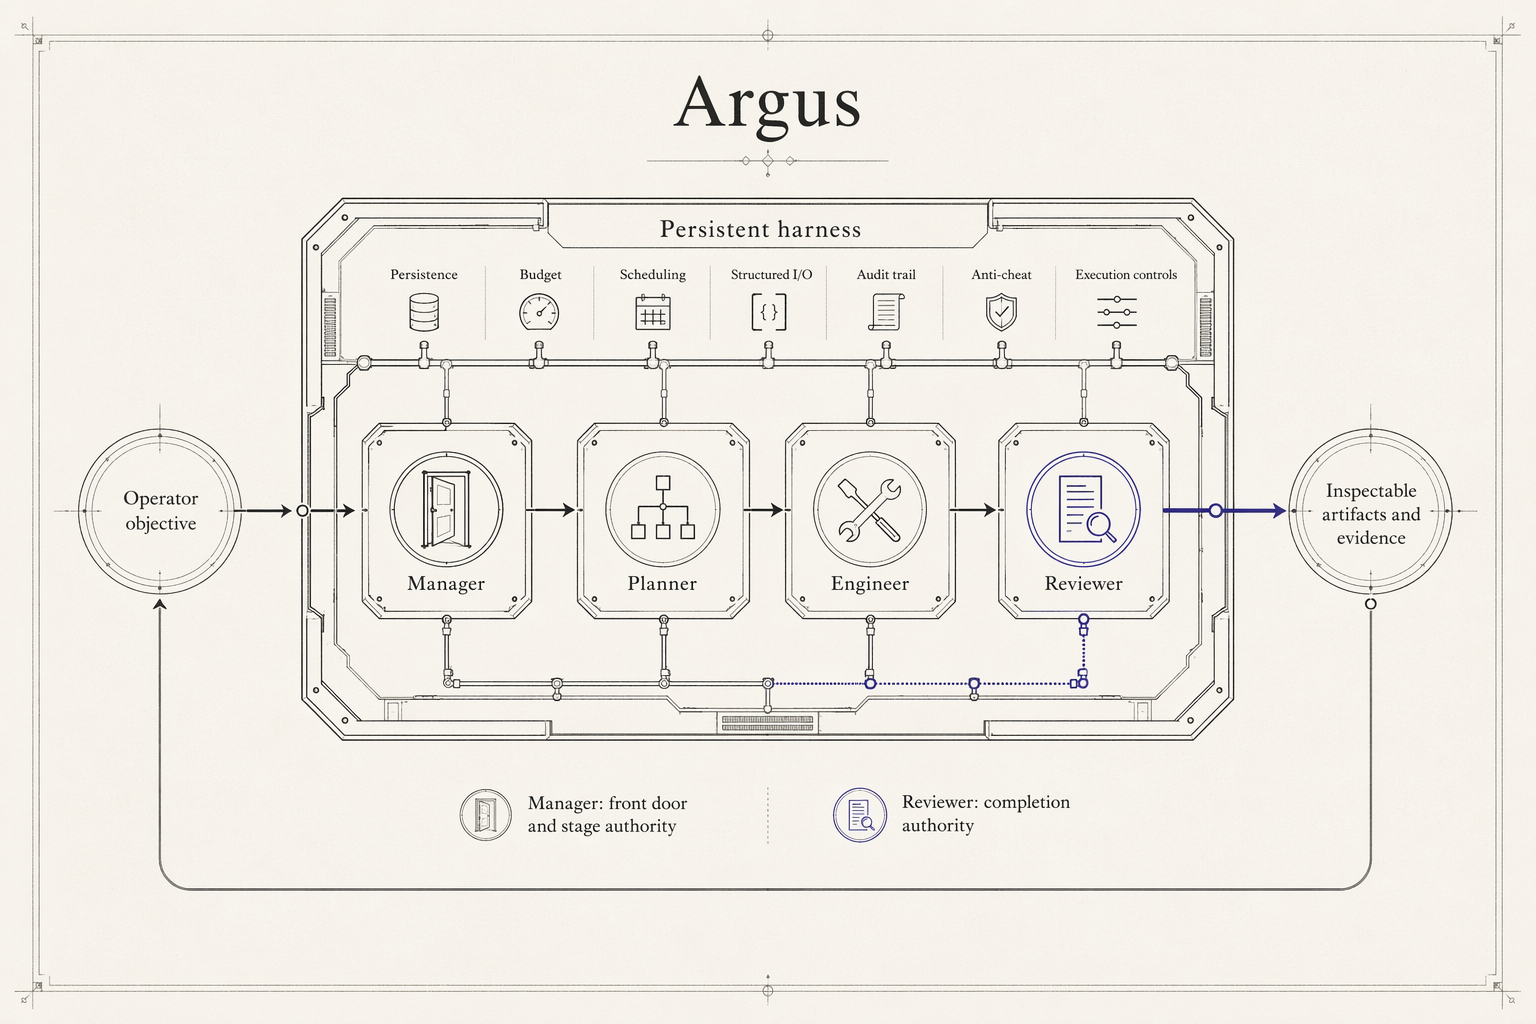
\includegraphics[width=0.82\textwidth]{figures/argus_architecture.png}
\caption{System schematic (not a measured performance plot) of the Argus
architecture: an operator objective enters a persistent, domain-agnostic
harness; the Manager, Planner, Engineer, and Reviewer sit inside it as the
four roles that make every research judgment; and inspectable artifacts and
evidence exit back to the operator.}
\label{fig:architecture}
\end{figure}

\subsection{Manager --- front door and stage authority}

The Manager is the single entry point for the operator. When free-form text
arrives, one grounded model call --- not a keyword match --- decides whether it is
chat or a task, selects the vertical (task shape) or authors a new data domain,
and commits that choice durably so the rest of the engine trusts it without
re-classifying. The Manager is also the \emph{sole} authority for pipeline-stage
transitions: it owns the \code{current\_stage} field, and Planner, Engineer, and
Reviewer may only \emph{advise} a stage change, never write it themselves. It has
its own backend and model configuration and appears alongside the other three
roles in the operator's cockpit. Crucially, the Manager never judges whether a
result is a win and never runs planning loops --- it divides the task and hands
the current stage to the Planner.

\subsection{Planner (L4) --- forward scheduling}

The Planner is the continuous scheduler. When the backlog empties in continuous
mode, it proposes the next unit of work. It also provides a completion
safeguard: if it prematurely reports a project ``done'' while a full-pipeline
completion has not yet been certified, the supervisor \emph{replaces} that verdict
with an explicit \code{scope:final\_submission} certification task and hands it
back to the Reviewer. This safeguard is driven by an explicit configuration flag,
not by inspecting the objective text. The retired L3 ``critic'' round-polishing
layer no longer exists; all acceptance flows to the Reviewer.

\subsection{Engineer (L1) --- one round of real work}

The Engineer executes a single round against real hardware and real tools:
literature search, code, experiments, or manuscript writing. It shares a working
directory with the Reviewer, so the Reviewer can inspect exactly what was
produced. The Engineer's round loop is where most reliability machinery lives
(Section~\ref{sec:reliability}): backend-failure recovery, session continuity,
context-pressure handling, and the background-subagent cadence wait. The
Engineer's prompt is kept intentionally light --- the current task, the original
objective, the matched or freshly distilled skill, the Reviewer's concrete next
step, and turn discipline --- so it is not buried under boilerplate.

\subsection{Reviewer (L2) --- the sole authority on ``done''}

The Reviewer is the completion authority, and there is no separate hardcoded
completion gate anywhere in the system. Each round it inspects the Engineer's
output against a structured stage checklist and returns one of three verdicts:
\code{done} (with an optional certification of a verified achievement),
\code{continue} (with a concrete next step for the Engineer), or \code{blocked}
(with the binding constraint). Because the Reviewer runs in the same work-tree
and is given the mission's execution log with grep recipes, it can audit
\emph{how} a result was produced --- catching a hardcoded answer, a skipped step,
or a faked metric --- rather than trusting the Engineer's summary. The Reviewer
also authors the curated working-memory checkpoint and labels each round's
decision-progress class, both described in Section~\ref{sec:reliability}.

\begin{callout}[Why ``done'' has exactly one owner]
Premature acceptance is a defining failure of autonomous agents. Argus answers it
structurally: completion is a \emph{single} structured verdict from a role that
sees the artifacts and the execution log, not a self-report from the role that
did the work, and not a keyword the harness fished out of a summary. If the
Reviewer is wrong, that is a model-quality limitation
(Section~\ref{sec:limitations}) --- but the authority is never ambiguous.
\end{callout}

\subsection{The harness beneath the roles}

Underneath the four roles sits the domain-agnostic core: budget and pricing,
persistence and paths, structured I/O ports, daemon locks, and the single
anti-stuck mechanism (regime-jump), which detects saturation with a dumb counter,
asks the Planner to judge whether to jump, and enforces a never-cleared forbidden
ledger --- failing soft to a no-op if anything goes wrong. Per-task shapes live in
pluggable \emph{verticals} (nanochat, nanoGPT speedrun, KernelBench, research, and
others), each supplying its role banner, completion gate, and strategy pool. The
outer \code{LifeSupervisor} is the 7$\times$24 loop: it claims backlog items,
injects a non-authoritative memory prelude without polluting the raw objective,
runs the mission, accounts cost against budget gates, and writes the journal.
State is persisted per project under a global root, so a daemon can be stopped,
upgraded, and resumed at a clean mission boundary without re-invoking the
Manager.
